\documentclass[11pt]{article}

\usepackage[T1]{fontenc}
\usepackage[utf8]{inputenc}
\usepackage{lmodern}
\usepackage[margin=1in]{geometry}
\usepackage{amsmath,amssymb,amsthm,mathtools}
\usepackage{booktabs}
\usepackage{array}
\usepackage{longtable}
\usepackage{enumitem}
\usepackage{float}
\usepackage{hyperref}
\usepackage[nameinlink,noabbrev]{cleveref}
\usepackage{tikz}
\usetikzlibrary{positioning,arrows.meta,shapes.geometric,fit}

\hypersetup{
  colorlinks=true,
  linkcolor=blue,
  citecolor=blue,
  urlcolor=blue
}

\newcommand{\R}{\mathbb{R}}
\newcommand{\Pcal}{\mathcal{P}}
\newcommand{\Wtwo}{W_2}
\newcommand{\dd}{\mathrm{d}}
\newcommand{\supp}{\operatorname{supp}}
\newcommand{\E}{\mathbb{E}}

\title{LaTeX Reading Review:\\A Mean Field View of the Landscape of Two-Layer Neural Networks}
\author{OpenAI Codex}
\date{\today}

\begin{document}
\maketitle
\tableofcontents

\section{Paper Metadata and Overview}

\paragraph{Reference.}
Song Mei, Andrea Montanari, and Phan-Minh Nguyen,
\emph{A mean field view of the landscape of two-layer neural networks},
PNAS 115(33):E7665--E7671, 2018 \cite{mei2018meanfield}.

\paragraph{Main problem.}
The paper studies two-layer networks trained by stochastic gradient descent (SGD) in the population setting. The main claim is that, in a suitable large-width / small-step-size regime, the empirical parameter distribution evolves according to a nonlinear PDE. This PDE is a Wasserstein gradient flow, and that description simplifies the loss-landscape analysis.

\paragraph{Core mathematical objects.}
The network prediction is
\begin{equation}
\hat y(x;\theta)=\frac{1}{N}\sum_{i=1}^N \sigma_*(x;\theta_i),
\end{equation}
with population risk
\begin{equation}
R_N(\theta)=\E\bigl[(y-\hat y(x;\theta))^2\bigr].
\end{equation}
After rewriting the risk in terms of the empirical measure
\(
\hat \rho^{(N)} = N^{-1}\sum_{i=1}^N \delta_{\theta_i},
\)
the paper introduces the mean-field functional
\begin{equation}
R(\rho)=R_\# + 2\int V(\theta)\,\rho(\dd \theta)
+ \int U(\theta_1,\theta_2)\,\rho(\dd\theta_1)\rho(\dd\theta_2).
\end{equation}
The corresponding distributional dynamics (DD) is
\begin{equation}
\partial_t \rho_t = 2\xi(t)\,\nabla_\theta \cdot \Bigl(\rho_t \nabla_\theta \Psi(\theta;\rho_t)\Bigr),
\qquad
\Psi(\theta;\rho)=V(\theta)+\int U(\theta,\theta')\,\rho(\dd\theta').
\end{equation}

\paragraph{High-level message.}
The proof spine has three layers:
\begin{enumerate}[label=\arabic*.]
\item rewrite the finite-width problem as an empirical-measure problem;
\item show SGD converges to a PDE by a propagation-of-chaos argument;
\item analyze the PDE rather than the original nonconvex optimization problem.
\end{enumerate}
The PDE can be studied using gradient-flow tools and, in some examples, yields near-global convergence guarantees.

\paragraph{Role of the Supplementary Information.}
The Supplementary Information is not optional here. It contains most of the formal proof architecture: Corollary~2.1, Lemmas in Sections~3--6, the proof of Theorem~3, and the detailed PDE / free-energy arguments that support Theorems~4--7.

\section{Dependency Graph}

\begin{figure}[H]
\centering
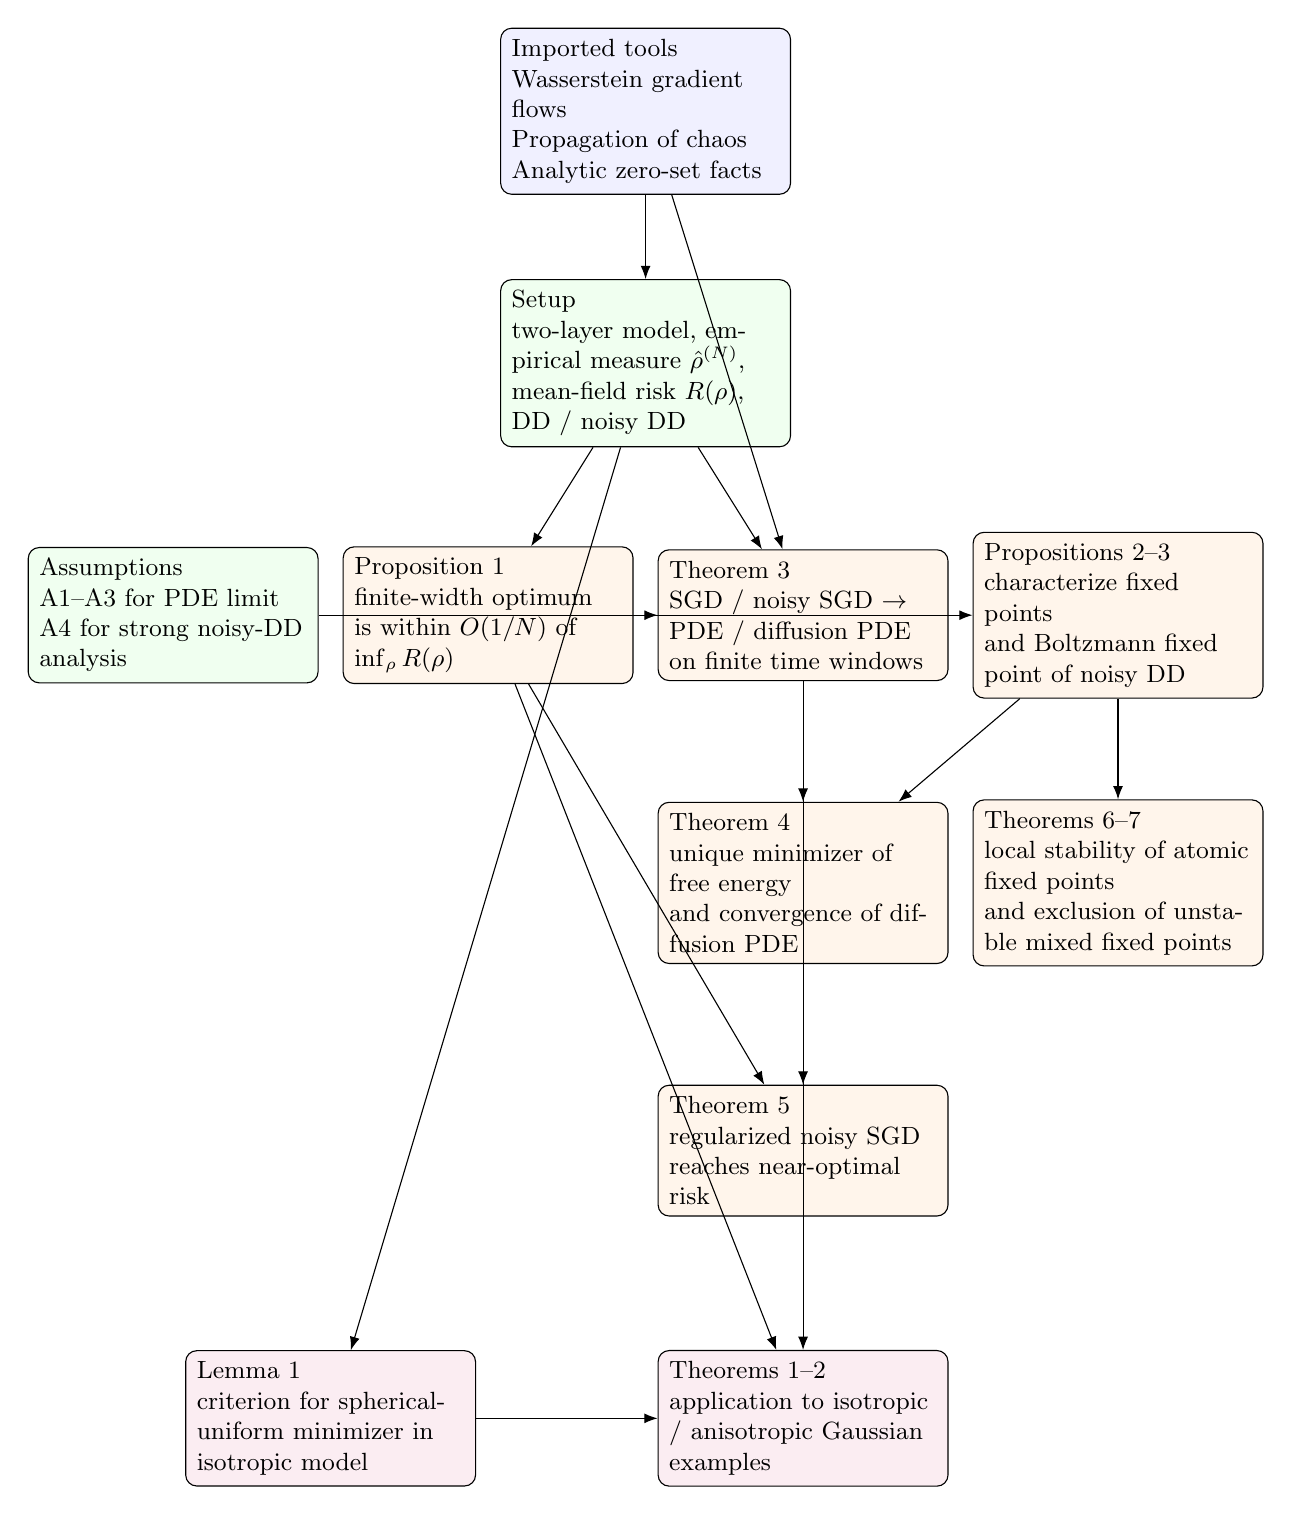
\begin{tikzpicture}[
  >=Latex,
  box/.style={
    draw,
    rounded corners,
    align=left,
    text width=3.4cm,
    font=\small,
    inner sep=4pt
  },
  imp/.style={box, fill=blue!6},
  core/.style={box, fill=green!6},
  res/.style={box, fill=orange!8},
  ex/.style={box, fill=purple!7}
]
\node[imp]  (tools)  at (0, 0)   {Imported tools\\Wasserstein gradient flows\\Propagation of chaos\\Analytic zero-set facts};
\node[core] (setup)  at (0,-3.2) {Setup\\two-layer model, empirical measure $\hat\rho^{(N)}$, mean-field risk $R(\rho)$, DD / noisy DD};
\node[core] (assump) at (-6.0,-6.4) {Assumptions\\A1--A3 for PDE limit\\A4 for strong noisy-DD analysis};
\node[res]  (prop1)  at (-2.0,-6.4) {Proposition 1\\finite-width optimum is within $O(1/N)$ of $\inf_\rho R(\rho)$};
\node[res]  (thm3)   at (2.0,-6.4) {Theorem 3\\SGD / noisy SGD $\to$ PDE / diffusion PDE on finite time windows};
\node[res]  (prop23) at (6.0,-6.4) {Propositions 2--3\\characterize fixed points\\and Boltzmann fixed point of noisy DD};
\node[res]  (thm4)   at (2.0,-9.8) {Theorem 4\\unique minimizer of free energy\\and convergence of diffusion PDE};
\node[res]  (thm67)  at (6.0,-9.8) {Theorems 6--7\\local stability of atomic fixed points\\and exclusion of unstable mixed fixed points};
\node[res]  (thm5)   at (2.0,-13.2) {Theorem 5\\regularized noisy SGD reaches near-optimal risk};
\node[ex]   (lemma1) at (-4.0,-16.6) {Lemma 1\\criterion for spherical-uniform minimizer in isotropic model};
\node[ex]   (thm12)  at (2.0,-16.6) {Theorems 1--2\\application to isotropic / anisotropic Gaussian examples};

\draw[->] (tools) -- (setup);
\draw[->] (setup) -- (prop1);
\draw[->] (setup) -- (thm3);
\draw[->] (tools) -- (thm3);
\draw[->] (assump) -- (thm3);
\draw[->] (assump) -- (prop23);
\draw[->] (thm3) -- (thm4);
\draw[->] (prop23) -- (thm4);
\draw[->] (thm4) -- (thm5);
\draw[->] (prop1) -- (thm5);
\draw[->] (prop23) -- (thm67);
\draw[->] (setup) -- (lemma1);
\draw[->] (lemma1) -- (thm12);
\draw[->] (thm3) -- (thm12);
\draw[->] (prop1) -- (thm12);
\end{tikzpicture}
\caption{Main proof spine of \cite{mei2018meanfield}. The central transition is from finite-width SGD to distributional dynamics, after which the analysis moves to fixed points, free energy, and example-specific PDE reductions. A few logically true but visually redundant edges are omitted so the main proof spine remains readable.}
\end{figure}

\paragraph{How to read the graph.}
The paper's most important move is Theorem~3: once SGD is approximated by DD, the optimization problem is replaced by the study of a measure-valued flow. The noisy branch (Proposition~3 $\to$ Theorem~4 $\to$ Theorem~5) gives the cleanest generic convergence result. The noiseless branch (Propositions~2, Theorems~6--7) gives a weaker but structurally informative picture of stable and unstable fixed points.

\section{Key Mathematical Assumptions}

\subsection*{Population-risk and one-pass setting}
The paper works in the population setting with i.i.d.\ training samples and explicitly adopts the \emph{One-Pass Assumption}: examples are not revisited. SGD is written with step size
\(
s_k = \varepsilon \,\xi(k\varepsilon).
\)
This scaling is what permits a continuum-time limit.

\subsection*{Main regularity assumptions in the paper}
The generic PDE-limit results are stated under assumptions A1--A4.
\begin{itemize}[leftmargin=1.5em]
\item \textbf{A1.} $\xi$ is bounded and Lipschitz, with $\int_0^\infty \xi(t)\,\dd t=\infty$.
\item \textbf{A2.} The activation $\sigma_*(x;\theta)$ is bounded, with sub-Gaussian gradient in $\theta$; labels are bounded.
\item \textbf{A3.} $\nabla V$ and $\nabla_1 U$ are bounded and Lipschitz.
\item \textbf{A4.} For the noisy-DD convergence theory, $V$ and $U$ are $C^4$ with bounded derivatives up to the stated order.
\end{itemize}

\subsection*{Two central PDEs}
The \emph{distributional dynamics} (noiseless mean-field limit) is
\begin{equation}
\partial_t \rho_t
=
2\xi(t)\,\nabla_\theta \cdot \Bigl(\rho_t \nabla_\theta \Psi(\theta;\rho_t)\Bigr),
\qquad
\Psi(\theta;\rho)=V(\theta)+\int U(\theta,\theta')\,\rho(\dd\theta').
\end{equation}
The \emph{diffusion DD} for noisy / regularized SGD has the schematic form
\begin{equation}
\partial_t \rho_t
=
2\xi(t)\,\nabla_\theta \cdot \Bigl(\rho_t \nabla_\theta \Psi_\lambda(\theta;\rho_t)\Bigr)
 + 2\xi(t)\beta^{-1}\Delta_\theta \rho_t,
\end{equation}
where $\beta$ is inverse temperature and $\lambda$ is the quadratic regularization strength.

\subsection*{Why these assumptions matter}
The assumptions are not cosmetic. A1--A3 are used to show existence / uniqueness of the PDE and to control the finite-time approximation error in Theorem~3. A4 is what allows the stronger free-energy analysis that yields Theorems~4--5. In short:
\begin{itemize}[leftmargin=1.5em]
\item A1--A3 support the \emph{PDE limit};
\item A4 supports the \emph{global convergence of the noisy PDE}.
\end{itemize}

\section{Key Claims and Results}

\subsection*{Problem formulation}
The two-layer model is
\begin{equation}
\hat y(x;\theta)=\frac{1}{N}\sum_{i=1}^N \sigma_*(x;\theta_i),
\end{equation}
and the population square-loss risk can be rewritten as
\begin{equation}
R_N(\theta)
=
R_\# + \frac{2}{N}\sum_{i=1}^N V(\theta_i)
+ \frac{2}{N^2}\sum_{i,j=1}^N U(\theta_i,\theta_j).
\end{equation}
This motivates the mean-field functional
\begin{equation}
R(\rho)=R_\# + 2\int V(\theta)\,\rho(\dd\theta)
+ \int U(\theta_1,\theta_2)\,\rho(\dd\theta_1)\rho(\dd\theta_2).
\end{equation}

\subsection*{Main theorem-level results from the paper}

\paragraph{Lemma 1.}
For the isotropic Gaussian example, this gives a criterion for when the uniform measure on a sphere of radius $r_*$ is a global minimizer of the reduced risk. This is the first concrete bridge from the abstract mean-field risk to an explicit optimizer in a model.

\paragraph{Theorem 1.}
In the isotropic Gaussian classification model, for good initialization and large enough dimension / width, SGD reaches risk within $\eta$ of the global optimum after a finite scaled time window. The key message is not just convergence, but convergence with sample complexity linear in dimension and independent of width once width is large enough.

\paragraph{Theorem 2.}
An analogous near-optimal SGD result holds for anisotropic Gaussian classification, where the task involves recovering a relevant subspace. This shows the framework is not restricted to a fully symmetric toy problem.

\paragraph{Theorem 3.}
This is the paper's central structural theorem: SGD and noisy SGD converge to the corresponding PDEs on finite time intervals. Formally, the empirical measure of parameters converges weakly to the solution of DD / diffusion DD. This is the propagation-of-chaos step that converts the optimization analysis into PDE analysis.

\paragraph{Proposition 1.}
The finite-width optimum differs from the mean-field optimum by at most $O(1/N)$ under a mild moment condition. This justifies using $\inf_\rho R(\rho)$ as a proxy for the large-width optimum.

\paragraph{Propositions 2 and 3.}
These characterize fixed points of the noiseless and noisy distributional dynamics. Proposition~2 gives the zero-current condition for noiseless DD. Proposition~3 gives the Boltzmann fixed-point formula
\begin{equation}
\rho_*(\theta)=\frac{1}{Z(\beta)}\exp\{-\beta \Psi_\lambda(\theta;\rho_*)\},
\end{equation}
for the noisy regularized flow.

\paragraph{Theorem 4.}
Under A1--A4 and $\lambda>0$, the free energy has a unique minimizer $\rho_{\beta,\lambda}^*$ and the diffusion PDE converges to it. This is the cleanest generic asymptotic result in the paper.

\paragraph{Theorem 5.}
Regularized noisy SGD inherits the PDE convergence and achieves near-optimal regularized risk. This is the main generic algorithmic corollary.

\paragraph{Theorems 6 and 7.}
These analyze noiseless fixed points. Theorem~6 gives a Hessian-based local stability condition for an atomic fixed point $\delta_{\theta^*}$: positive definite local Hessian implies local exponential convergence. Theorem~7 gives a converse instability-type statement for certain mixed fixed points with a saddle direction.

\subsection*{Free-energy identity}
One of the most important formulas in the paper is the free-energy dissipation law for the noisy PDE:
\begin{equation}
\label{eq:free-energy-note}
\frac{\dd}{\dd t}F_{\beta,\lambda}(\rho_t)
=
-2\xi(t)\int
\bigl\|\nabla_\theta \bigl(\Psi_\lambda(\theta;\rho_t)+\beta^{-1}\log \rho_t(\theta)\bigr)\bigr\|_2^2\,
\rho_t(\theta)\,\dd\theta.
\end{equation}
This is the backbone of Theorem~4. It is the point where the Wasserstein gradient-flow structure becomes operational.

\section{Proof-Sketch Architecture for the Main Results}

\subsection*{Theorem 3: SGD $\to$ PDE}
\begin{enumerate}[label=\arabic*.]
\item Rewrite SGD in terms of the empirical measure of particles / parameters.
\item Introduce the nonlinear McKean--Vlasov-style dynamics whose law solves the PDE.
\item Compare discrete SGD trajectories with the nonlinear dynamics trajectory-by-trajectory.
\item Control the discrepancy using boundedness / Lipschitz assumptions and concentration for martingale-difference terms.
\item Conclude weak convergence of empirical measures to $\rho_t$.
\end{enumerate}
\paragraph{Uses.}
A1--A3, propagation-of-chaos ideas, and the Supplementary Information Lemmas~3.1--3.4. This theorem is later used by Theorems~1, 2, and 5.

\subsection*{Theorem 4: convergence of the noisy PDE}
\begin{enumerate}[label=\arabic*.]
\item Define the regularized free energy $F_{\beta,\lambda}(\rho)$.
\item Prove the dissipation identity along the diffusion PDE.
\item Use that identity to show every long-time limit must satisfy the Boltzmann fixed-point equation.
\item Use convexity / regularization to show uniqueness of the minimizer and hence identify the limit.
\end{enumerate}
\paragraph{Uses.}
Proposition~3, A1--A4, and the free-energy framework imported from Wasserstein-gradient-flow theory. Theorem~5 depends on this result.

\subsection*{Theorem 5: noisy SGD reaches near-optimal regularized risk}
\begin{enumerate}[label=\arabic*.]
\item Apply Theorem~3 to replace finite-width noisy SGD by diffusion DD on a finite time window.
\item Apply Theorem~4 to show the PDE reaches the unique free-energy minimizer.
\item Compare the free-energy minimizer to the finite-width optimum using Proposition~1 and the entropy / regularization error terms.
\end{enumerate}
\paragraph{Uses.}
This is the paper's main generic optimization conclusion. Its proof is modular: PDE limit + PDE convergence + mean-field approximation.

\subsection*{Theorems 6 and 7: local structure of noiseless fixed points}
\paragraph{Theorem 6.}
The proof expands $\Psi(\theta;\rho)$ near a candidate atomic fixed point and checks the local Hessian
\begin{equation}
H_0(\rho^*)=\nabla^2 V(\theta^*)+\int \nabla^2_{1,1}U(\theta^*,\theta)\,\rho^*(\dd\theta).
\end{equation}
If $\lambda_{\min}(H_0)>0$, then the local drift points inward and the dynamics contracts toward $\delta_{\theta^*}$.

\paragraph{Theorem 7.}
The argument is essentially an instability exclusion: if a mixed fixed point has a negative Hessian direction and enough nearby mass, then a bounded-density initial condition cannot converge to it. The paper states this as a structural obstruction rather than as a full global classification theorem.

\subsection*{Theorems 1 and 2: example-specific convergence}
The examples reduce the PDE to lower-dimensional radial or symmetry-reduced equations. Then the authors identify good minimizers and show that the corresponding PDE trajectory reaches them under suitable initialization. The general Theorem~3 is what lifts these PDE conclusions back to finite-width SGD.

\paragraph{Important uncertainty note.}
The exact dependence of the convergence time $T$ on dimension and tolerance is not resolved in the generic theorems. The paper is explicit that the proof does not give a satisfactory estimate in full generality.

\section{Theorem/Lemma Dependency Tracking}

\begin{longtable}{>{\raggedright\arraybackslash}p{2.2cm} >{\raggedright\arraybackslash}p{4.0cm} >{\raggedright\arraybackslash}p{4.2cm} >{\raggedright\arraybackslash}p{4.2cm}}
\toprule
Item & One-line meaning & Depends on & Used later \\
\midrule
\endfirsthead
\toprule
Item & One-line meaning & Depends on & Used later \\
\midrule
\endhead
Lemma 1 & Criterion for spherical-uniform global minimizer in isotropic model & Reduced isotropic risk; model symmetry & Theorem 1 and the example analysis \\
Theorem 1 & Near-optimal SGD in isotropic Gaussian model & Reduced PDE analysis, good initialization, Theorem 3 (explicitly or implicitly) & Main application result \\
Theorem 2 & Near-optimal SGD in anisotropic Gaussian model & Reduced PDE analysis, symmetry reduction, Theorem 3 & Main application result \\
Proposition 1 & $\inf_\theta R_N(\theta)$ is close to $\inf_\rho R(\rho)$ & Mean-field risk representation; moment bound & Theorems 4--5; example interpretation \\
Theorem 3 & Empirical SGD measure converges to DD / diffusion DD & A1--A3; nonlinear dynamics; Supplementary Section 3 & Theorems 1, 2, 5 \\
Proposition 2 & Characterizes fixed points of noiseless DD & DD as a continuity equation; zero-current condition & Theorems 6--7 \\
Proposition 3 & Unique Boltzmann fixed point for noisy DD & Free-energy structure; regularity; diffusion PDE & Theorem 4 \\
Theorem 4 & Diffusion DD converges to unique free-energy minimizer & Proposition 3; A1--A4; dissipation identity \eqref{eq:free-energy-note} (informal reference) & Theorem 5 \\
Theorem 5 & Regularized noisy SGD achieves near-optimal regularized risk & Theorems 3--4; Proposition 1 & Generic algorithmic conclusion \\
Theorem 6 & Positive Hessian implies local stability of atomic fixed point & Proposition 2; local Hessian $H_0$ & Noiseless asymptotic interpretation \\
Theorem 7 & Certain mixed fixed points are unstable for bounded-density initials & Theorem 6-type Hessian geometry; additional level-set assumptions & Noiseless asymptotic interpretation \\
Corollary 2.1 (SI) & Analytic minimizers are either flat or supported on a null set & Analyticity of $V,U$ and minimizer condition & Conceptual explanation for singular minimizers \\
Lemmas 3.1--3.4 (SI) & PDE continuity and trajectory-comparison estimates & A1--A3, concentration bounds & Proof of Theorem 3 \\
\bottomrule
\end{longtable}

\paragraph{Internal vs.\ imported dependencies.}
\begin{itemize}[leftmargin=1.5em]
\item \textbf{Paper-internal backbone:} Proposition~1, Theorem~3, Propositions~2--3, Theorems~4--7.
\item \textbf{Imported background tools:} Wasserstein gradient-flow framework \cite{jordan1998variational,ambrosio2008gradient}; propagation of chaos \cite{sznitman1991topics}.
\item \textbf{Example-specific analysis:} Lemma~1 and the reduced PDEs for isotropic / anisotropic Gaussian models.
\item \textbf{Not part of the proof backbone:} the numerical PDE solutions in the figures. They illustrate the theory, but they do not prove the main abstract convergence statements.
\end{itemize}

\paragraph{Uncertainty marker.}
The paper does not always spell out every proof dependency in theorem-by-theorem style. In particular, the exact dependency of Theorems~1--2 on Theorem~4 is partly inferred from the shared mean-field philosophy and not asserted as a direct proof chain.

\section{Prerequisite Knowledge and Imported Tools}

\subsection*{Wasserstein gradient flows}
The paper repeatedly uses the idea that the limiting PDE is a gradient flow on the metric space $(\Pcal(\R^D), \Wtwo)$. The relevant imported viewpoint is the Jordan--Kinderlehrer--Otto / Ambrosio--Gigli--Savar\'e framework \cite{jordan1998variational,ambrosio2008gradient}. This is not re-proved in the paper, but it strongly shapes how the PDE is interpreted.

\subsection*{Propagation of chaos}
The step from finite-width SGD to a measure-valued nonlinear limit is an instance of propagation of chaos \cite{sznitman1991topics}. The paper's proof is largely self-contained, but this is the conceptual background.

\subsection*{Measure-valued PDEs}
The distributional dynamics is interpreted weakly in the space of probability measures. A reader should already be comfortable with continuity equations, weak solutions, and measure-valued evolutions.

\subsection*{Classical optimization and SGD scaling}
The paper assumes familiarity with SGD in the small-step-size regime and with the idea that a discrete optimization algorithm can converge to an ODE/PDE under scaling.

\subsection*{Example-specific prerequisites}
The isotropic and anisotropic Gaussian examples use symmetry reduction. The reader should be comfortable with:
\begin{itemize}[leftmargin=1.5em]
\item radial distributions and rotational invariance;
\item reduced coordinates for anisotropic covariance structure;
\item basic sub-Gaussian concentration estimates.
\end{itemize}

\section{Section-by-Section Structural Notes}

\subsection*{Main paper}

\paragraph{Introduction and informal overview.}
The introduction does two things at once: it motivates the optimization question for two-layer networks, and it announces the PDE replacement of SGD as the central simplification. The ``informal overview'' is structurally important because it already gives the key formulas for $R_N$, $R(\rho)$, and the DD before the theorems appear.

\paragraph{Concrete examples.}
The isotropic Gaussian, anisotropic Gaussian, ReLU, and failure examples are not side material. They serve as demonstrations that the PDE viewpoint can both predict success and diagnose failure. The examples are also where the paper conveys intuition more clearly than in the generic theorems.

\paragraph{General results.}
This is the abstract core of the paper. Proposition~1 and Theorems~3--7 define the reusable mathematical package. If one only wants the proof architecture of the paper, this is the essential section in the main text.

\paragraph{Discussion and future directions.}
The discussion is modestly honest about what has and has not been proved. The PDE limit is strong, but the generic rates are incomplete, and the nicest convergence results require noisy / regularized dynamics. This section is useful because it tells the reader what not to overclaim.

\subsection*{Supplementary Information}

\paragraph{Section 2: static properties of $R(\rho)$.}
This section contains the mean-field variational backbone behind Proposition~1 and Corollary~2.1. It explains why minimizers can become singular and why the measure-valued perspective is nontrivial even though $R(\rho)$ looks convex-ish.

\paragraph{Section 3: dynamics and proof of Theorem 3.}
This is the most important supplement section mathematically. It contains the nonlinear dynamics representation, the continuity properties, and the trajectory-comparison lemmas that make the propagation-of-chaos argument work.

\paragraph{Sections 4 and 5: example-specific reduced analyses.}
These sections specialize the abstract machinery to the isotropic / anisotropic examples and related reduced PDEs. They are where one sees the practical analytical benefit of the mean-field reduction.

\paragraph{Section 6: noisy dynamics and free energy.}
This section contains the details behind the free-energy minimization, fixed points, and the noisy-DD convergence results. It is the technical foundation for Theorems~4--5.

\paragraph{Structural reading advice.}
If studying the paper for reuse rather than for every proof detail, the best order is:
\begin{enumerate}[label=\arabic*.]
\item read the informal overview for the main objects;
\item read the statements of Proposition~1 and Theorems~3--7;
\item read Supplementary Section~3;
\item read Supplementary Section~6;
\item only then revisit the example sections.
\end{enumerate}

\section{Reuse Notes and Open Questions}

\paragraph{Why this paper matters for our work.}
This paper is useful less because it solves two-layer networks completely, and more because it replaces parameter optimization by measure evolution. That shift is conceptually important for any architecture where the right large-scale object is not a vector of parameters but a distribution over architectural components.

\paragraph{Potential reuse directions.}
\begin{itemize}[leftmargin=1.5em]
\item The empirical-measure viewpoint may be relevant if we later want to study neural architectures whose effective state is a population over nodes, paths, or motifs.
\item The ``good initialization + PDE limit + PDE convergence'' proof pattern is a reusable template.
\item The Hessian-based stability criteria in Theorems~6--7 suggest a way to reason about stable versus unstable architectural regimes without solving the full finite system.
\end{itemize}

\paragraph{Open questions left by the paper.}
\begin{itemize}[leftmargin=1.5em]
\item Can the dependence of the convergence time on dimension and tolerance be made explicit in generic settings?
\item How much of the clean noisy-DD theory survives without regularization?
\item Can analogous PDE limits be developed for architectures with non-exchangeable geometric structure, where the parameter distribution is not permutation-symmetric?
\end{itemize}

\paragraph{Bottom line.}
The main reusable lesson is not ``SGD always works'' but rather: in some high-width regimes, the right object to analyze is a probability measure evolving under a gradient-flow PDE, and that object may have a much cleaner landscape than the original parameter system.


\bibliographystyle{plain}
\bibliography{references}

\end{document}
